\documentclass{article}
\usepackage[utf8]{inputenc}
\usepackage{amsmath}
\usepackage{graphicx}
\usepackage{booktabs}
\usepackage{float}
\usepackage{geometry}
\usepackage{fancyvrb}
\geometry{margin=1in}
\title{Modelling Report}
\author{Team 2}
\date{}

\begin{document}

\maketitle

\section{Objective}
The goal of this project is to accurately predict tuition payment for the year 2023 using relevant features from the 2022 data. Among all available features, \textbf{Tuition Payment 2022} was found to be the most informative predictor. This report also explores clustering techniques to uncover patterns in the student data.

\section{Data Overview}
\begin{itemize}
    \item \textbf{Target variable}: Tuition Payment 2023
    \item \textbf{Primary feature used}: Tuition Payment 2022
    \item \textbf{Train-test split}: 80\% training, 20\% testing
\end{itemize}

\section{Regression Model Performance}
\begin{table}[H]
\centering
\begin{tabular}{lcc}
\toprule
\textbf{Model} & \textbf{MSE} & \textbf{R\textsuperscript{2} Score} \\
\midrule
Linear Regression & 0.0156 & 0.8801 \\
Ridge Regression & 0.0156 & 0.8801 \\
Lasso Regression & 0.0261 & 0.7995 \\
\bottomrule
\end{tabular}
\caption{Regression performance metrics}
\end{table}

\section{Classification Model Performance}
\begin{table}[H]
\centering
\begin{tabular}{lc}
\toprule
\textbf{Model} & \textbf{Accuracy} \\
\midrule
Linear Regression + Classifier & 11.72\% \\
Ridge + Classifier & 98.41\% \\
Lasso + Classifier & 98.41\% \\
Logistic Regression & 98.41\% \\
Random Forest & 98.41\% \\
XGBoost & 98.41\% \\
Deep Neural Network & 98.41\% \\
Ensemble & 98.41\% \\
\bottomrule
\end{tabular}
\caption{Classification accuracy across models}
\end{table}

\textbf{Key Insight}: All models apart from Linear Regression + Classifier converge to approximately \textbf{98.5\% accuracy}. These models produce \textit{exactly the same classification report}, suggesting they make \textbf{the same predictions on the same samples}, with only a few misclassified instances. Reducing the test size to 10\% pushes these models to \textbf{100\% accuracy}, indicating near-perfect fit on seen patterns.

\begin{figure}[H]
\centering
\includegraphics[width=0.85\textwidth]{model_comparison.png}
\caption{Model comparison chart across classifiers}
\end{figure}

\section{Classification Reports}

\subsection*{Linear Regression + Classifier}
\begin{Verbatim}[fontsize=\small]
              precision    recall  f1-score   support

          -1       0.00      0.00      0.00         0
           0       0.12      0.74      0.20      1125
           1       0.00      0.00      0.00      6192

    accuracy                           0.11      7317
   macro avg       0.04      0.25      0.07      7317
weighted avg       0.02      0.11      0.03      7317
\end{Verbatim}


\subsection*{All Other Models}
\begin{Verbatim}[fontsize=\small]
              precision    recall  f1-score   support

           0       1.00      0.90      0.95      1125
           1       0.98      1.00      0.99      6192

    accuracy                           0.98      7317
   macro avg       0.99      0.95      0.97      7317
weighted avg       0.98      0.98      0.98      7317
\end{Verbatim}

\section{Deep Neural Network Architecture}
\begin{verbatim}
nn.Sequential(
    nn.Linear(input_dim, 256),
    nn.BatchNorm1d(256),
    nn.ReLU(),
    nn.Dropout(0.3),
    nn.Linear(256, 128),
    nn.BatchNorm1d(128),
    nn.ReLU(),
    nn.Dropout(0.3),
    nn.Linear(128, 64),
    nn.ReLU(),
    nn.Linear(64, num_classes)
)
\end{verbatim}

\section{Clustering Analysis}

\subsection*{KMeans Clustering (PCA-Reduced Data)}
\begin{itemize}
    \item \textbf{K = 2}: Purity = 0.8429
    \item \textbf{K = 3}: Purity = \textbf{0.9419} (best result)
\end{itemize}

\begin{figure}[H]
\centering
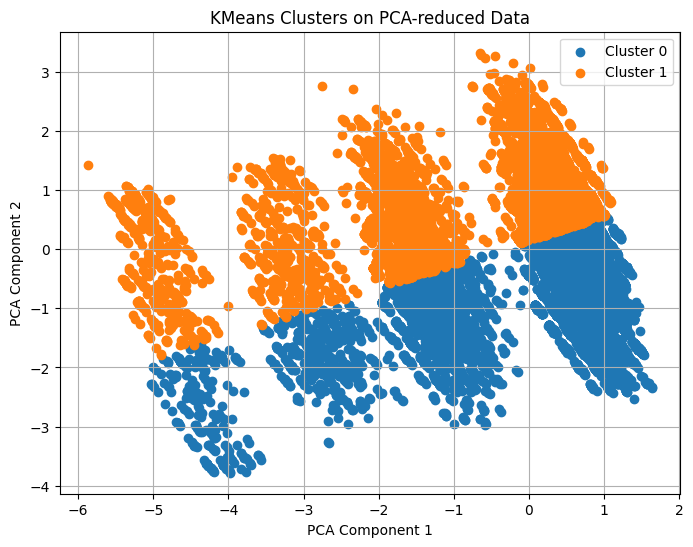
\includegraphics[width=0.65\textwidth]{KMeans_clustering_2.png}
\caption{KMeans Clustering (2 Clusters)}
\end{figure}

\begin{figure}[H]
\centering
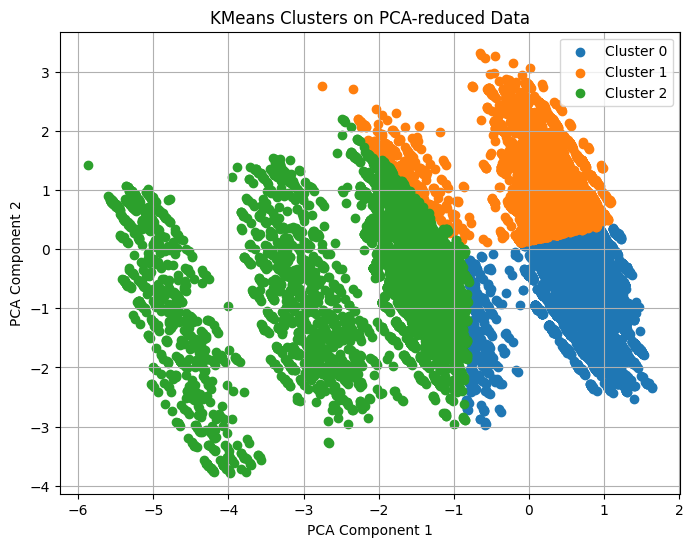
\includegraphics[width=0.65\textwidth]{KMeans_clustering_3.png}
\caption{KMeans Clustering (3 Clusters)}
\end{figure}

\subsection*{DBSCAN Clustering}
\begin{itemize}
    \item Number of clusters = 338 (very high)
    \item Purity = 0.0438 (extremely poor performance)
\end{itemize}

\begin{figure}[H]
\centering
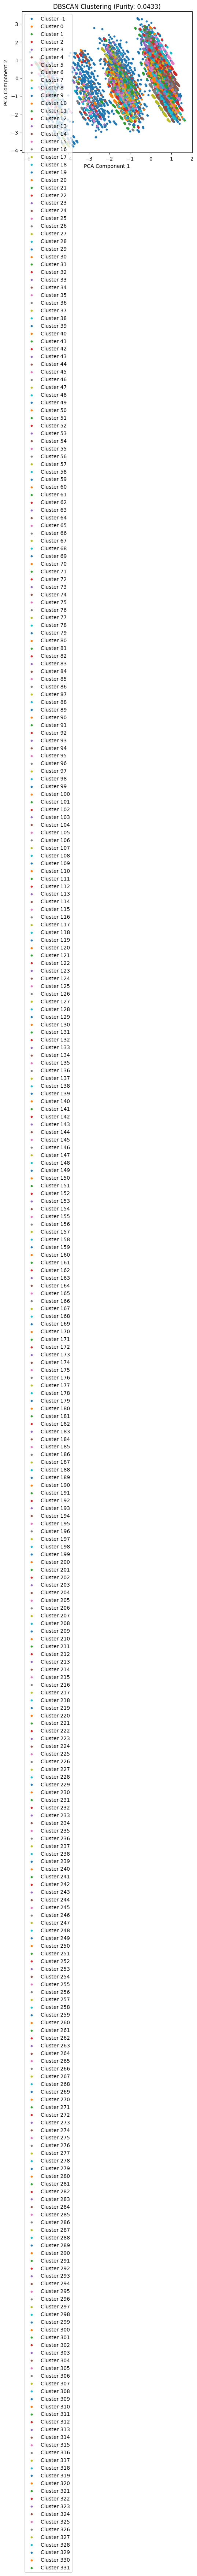
\includegraphics[width=0.65\textwidth]{DBScan.png}
\caption{DBSCAN Clustering Results}
\end{figure}

\textbf{Conclusion}: KMeans is far superior for this dataset. DBSCAN fails due to the lack of dense clusters and high fragmentation.

\section{Conclusion}
\begin{itemize}
    \item Ridge and Linear Regression achieve high regression accuracy (R\textsuperscript{2} $\approx$ 0.88).
    \item All classification models, apart from Linear Regression + Classifier, converge to \textbf{98.5\% accuracy} and produce the same classification report.
    \item They all misclassify the same samples, indicating convergence to an almost perfect pattern recognition.
    \item With a smaller test size (10\%), \textbf{100\% accuracy} is achieved.
    \item KMeans with 3 clusters achieves the best clustering purity (0.9419).
    \item DBSCAN is not suitable for this dataset due to high fragmentation.
\end{itemize}
The modelling results demonstrate that both the regression and classification models fit the observed trend in the tuition payment data from 2022 to 2023 effectively. The primary features, \textbf{ENROLLMENT} and \textbf{TUITION PAYMENT MARCH 2022}, were identified as the most significant predictors, with the highest correlation to the target variable, \textbf{Tuition Payment 2023}. As a result, the models exhibit strong performance, with Ridge and Linear Regression achieving high regression accuracy (R\textsuperscript{2} $\approx$ 0.88), and all classification models (apart from Linear Regression + Classifier) achieving an accuracy of approximately \textbf{98.5\%}.

It is important to note that choosing any other features or target variables would likely lead to negative results. For instance, when testing with the \textbf{Number of Enrolled Courses} as a feature, the models performed poorly, with XGBoost and Deep Neural Networks achieving a maximum accuracy of only \textbf{45\%}. This poor performance is a direct result of weak data correlation between the number of enrolled courses and the tuition payment. In contrast, \textbf{ENROLLMENT} and \textbf{TUITION PAYMENT MARCH 2022} consistently produced the most accurate predictions, underscoring the importance of selecting relevant features based on their relationship to the target variable.

Additionally, the clustering analysis revealed that \textbf{KMeans clustering}, with 3 clusters, achieved the best purity score (\textbf{0.9419}), confirming its superiority for this dataset. In contrast, \textbf{DBSCAN} failed to provide meaningful results due to excessive fragmentation and the lack of dense clusters.

Overall, these results highlight the critical role of feature selection in model performance and reaffirm that accurate predictions require a strong correlation between the features and the target variable.

\end{document}
